\documentclass[a4paper]{article}

\usepackage[UTF8]{ctex}
\usepackage[a4paper,margin=1in]{geometry}
\usepackage{graphicx}
\usepackage{float}
\usepackage{listings}
\usepackage{longtable}
\usepackage{booktabs}
\usepackage{hyperref}
\usepackage{fancyhdr}
\usepackage{lastpage}
\usepackage{color}
\usepackage{indentfirst}        % 首段缩进
\setlength{\parindent}{2em}     % 缩进2字符
\usepackage{zhnumber}           % 中文编号
\usepackage[dvipsnames]{xcolor}

%\newcommand{\college}{中山大学计算机学院}
\newcommand{\projname}{数据库系统原理实验|实验七}
\newcommand{\reporttitle}{存储过程和函数实验}
\newcommand{\stuno}{23336179}
\newcommand{\authorname}{马福泉}
\newcommand{\major}{计算机科学与技术}
\newcommand{\adviser}{赖韩江}
\newcommand{\startdate}{2025年11月6日}
\newcommand{\labenddate}{2025年11月11日}
\newcommand{\labroom}{B202}

\pagestyle{fancy} % 使用 fancyhdr 风格
\fancyhf{}      % 清空默认的页眉页脚

% 设置页眉
\fancyhead[L]{\kaishu \projname}      % 左侧页眉显示项目名称
\fancyhead[C]{\kaishu \reporttitle}    % 中间页眉显示报告标题
\fancyhead[R]{\kaishu \authorname} % 右侧页眉显示作者姓名

% 设置页脚
\fancyfoot[C]{第 \thepage 页，共 \pageref{LastPage} 页} % 中间页脚显示页码

% 去除页眉页脚与正文之间的分隔线
\renewcommand{\headrulewidth}{0.4pt}
\renewcommand{\footrulewidth}{0pt}

% 设置文档背景颜色
\definecolor{mybgcolor}{RGB}{0, 0, 0} % 定义背景颜色
\definecolor{NavyBlue}{RGB}{0,0,128} % 添加颜色定义
% \pagecolor{mybgcolor} % 设置背景颜色

% listing 配置rust
% \lstdefinelanguage{Rust}{
%   keywords={fn, let, mut, struct, enum, impl, pub, use, mod, trait, where},
%   keywordstyle=\color{NavyBlue},
%   comment=[l]{//},
%   commentstyle=\color{gray},
% }
% \lstset{language=Rust}

\lstset{
  basicstyle=\ttfamily\small,
  keywordstyle=\color{NavyBlue},
  commentstyle=\color{gray},
  stringstyle=\color{red},
  showstringspaces=false,
  extendedchars=false, % 关键：不处理中文
  breaklines=true
}

\begin{document}

% 封面
\begin{titlepage}
    \centering
    
\includegraphics[width=10cm]{img/SYSULogo.png}

    \vspace{1em}
    %{\Large \college \par}
    \vspace{1em}
    {\Large \kaishu \projname \par}
    \vspace{3em}

    

    
    {\fontsize{40pt}{42pt}\kaishu \selectfont \boldmath \reporttitle\par}
    \vspace*{\fill}

    \begin{center}
    {\Large
    \makebox[5em][s]{学号}:\underline{\makebox[15em][c]{\kaishu \stuno}}\\[1em]
    \makebox[5em][s]{姓名}:\underline{\makebox[15em][c]{\kaishu \authorname}}\\[1em]
    \makebox[5em][s]{专业}:\underline{\makebox[15em][c]{\kaishu \major}}\\[1em]
    \makebox[5em][s]{课程教师}:\underline{\makebox[15em][c]{\kaishu \adviser}}\\[1em]
    \makebox[5em][s]{起始日期}:\underline{\makebox[15em][c]{\kaishu \startdate}}\\[1em]
    \makebox[5em][s]{结束日期}:\underline{\makebox[15em][c]{\kaishu \labenddate}}\\[1em]
    \makebox[5em][s]{实验地点}:\underline{\makebox[15em][c]{\kaishu \labroom}}
    }
    \end{center}

    \vspace*{\fill}
\end{titlepage}

% 目录
\tableofcontents
\newpage


\section{实验概述}
本实验旨在掌握数据库存储过程和函数的定义与使用。实验内容包括：

\begin{enumerate}
    \item \textbf{无参数的存储过程或函数} \\
    定义一个存储过程或函数，实现打印“本人学号+姓名”（如：张三+22111001）。
    \item \textbf{有参数的存储过程或函数}
    \begin{enumerate}
        \item 首先将数据库中的图书表 book\_price 更新为指定价格：
        \begin{center}
        \begin{tabular}{ccc}
        \toprule
        book\_id & book\_name & book\_price \\
        \midrule
        b0001 & SQL Server 2012宝典 & 98.00 \\
        b0002 & 职称英语专用教材 & 36.00 \\
        b0003 & 中国通史 & 57.00 \\
        b0004 & 丰子恺儿童文学选集 & 19.80 \\
        b0005 & 英语同义词辨析词典 & 63.50 \\
        b0006 & 数据库基础与应用 & 33.00 \\
        b0007 & 微积分初步 & 78.50 \\
        b0008 & ASP.NET从入门到精通 & 69.80 \\
        \bottomrule
        \end{tabular}
        \end{center}
        \item 定义一个存储过程或函数：找出某个同学（输入名字，如“谢嫣然”）所读的所有图书名。
        \item 定义一个存储过程或函数：如果图书的价格小于等于35元，增加图书的价格为 book\_price $\times$(1+discount)；如果图书价格大于55元，图书的价格打折，更改为 book\_price $\times$(1-discount)。注意：不要互相影响。例如 discount=0.9，30元的图书更新为 30$\times$(1+0.9)=57，到这里就结束，不要继续做 57$\times$(1-0.9)。
        
        % 插入导师关系表截图
        \item 导师关系表如下：
        \begin{figure}[H]
            \centering
            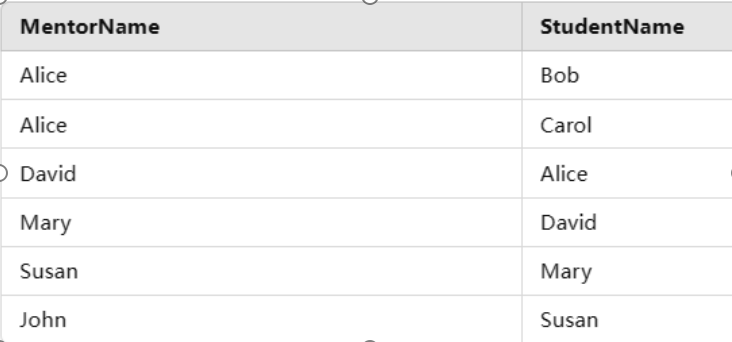
\includegraphics[width=0.8\textwidth]{img/advisor_table.png}
            \caption{导师关系表截图}
        \end{figure}
        
        \item 给定导师关系表，输入姓名，找出该学生的师承关系（导师、导师的导师、……），并返回所有相关导师的姓名。例如，输入 Mary，输出为 Susan, John。
    \end{enumerate}
    \item \textbf{游标} \\
    定义一个存储过程或函数，用游标的方式计算所有图书的总价。
\end{enumerate}

\section{实验报告}

\subsection{无参数的存储过程或函数}

\subsubsection{实验目标}
定义一个存储过程或函数，实现打印"本人学号+姓名"。

\subsubsection{代码实现}
\begin{lstlisting}[language=SQL]
CREATE FUNCTION GetStudentInfo()        -- 创建无参数函数，返回学号+姓名
RETURNS VARCHAR(50)
AS
BEGIN
    RETURN '马福泉+23336179'
END
GO
SELECT dbo.GetStudentInfo() AS StudentInfo;     -- 调用函数
\end{lstlisting}

\subsubsection{运行结果}
\begin{figure}[H]
    \centering
    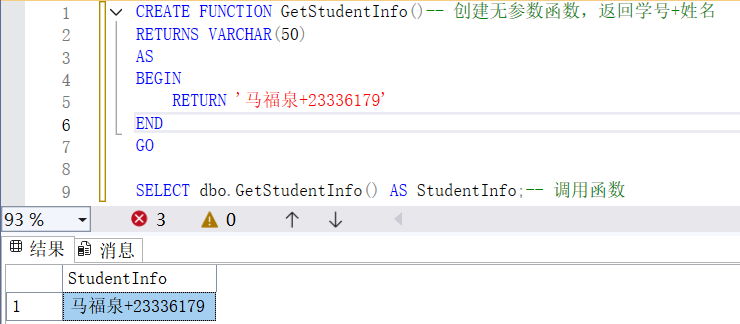
\includegraphics[width=0.8\textwidth]{img/result_1.png}
    \caption{无参数函数运行结果}
\end{figure}

\subsection{有参数的存储过程或函数}

\subsubsection{更新图书表价格}

\paragraph{实验目标}
将数据库中的图书表book\_price更新为指定价格。

\paragraph{代码实现}
\begin{lstlisting}[language=SQL]
UPDATE book SET book_price = 98.00 WHERE book_id = 'b0001';        -- 更新图书表价格
UPDATE book SET book_price = 36.00 WHERE book_id = 'b0002';
UPDATE book SET book_price = 57.00 WHERE book_id = 'b0003';
UPDATE book SET book_price = 19.80 WHERE book_id = 'b0004';
UPDATE book SET book_price = 63.50 WHERE book_id = 'b0005';
UPDATE book SET book_price = 33.00 WHERE book_id = 'b0006';
UPDATE book SET book_price = 78.50 WHERE book_id = 'b0007';
UPDATE book SET book_price = 69.80 WHERE book_id = 'b0008';

SELECT book_id, book_name, book_price FROM book;       -- 查看更新结果
\end{lstlisting}

\paragraph{运行结果}
\begin{figure}[H]
    \centering
    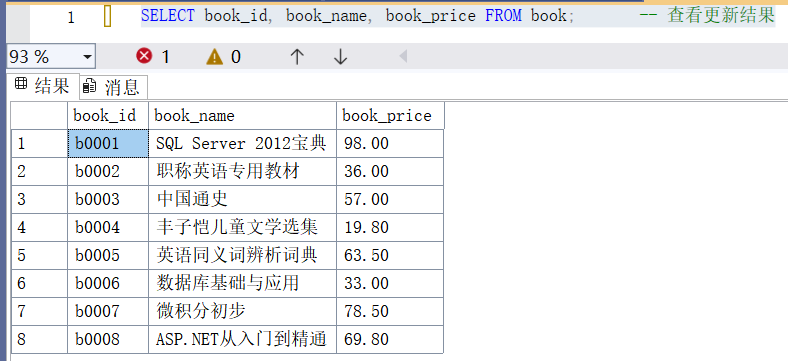
\includegraphics[width=0.8\textwidth]{img/result_2_1.png}
    \caption{图书表价格更新结果}
\end{figure}

\subsubsection{查找学生所读图书}

\paragraph{实验目标}
定义一个存储过程或函数，找出某个同学所读的所有图书名。

\paragraph{代码实现}
\begin{lstlisting}[language=SQL]
CREATE PROCEDURE GetStudentBooks
    @StudentName VARCHAR(50)
AS
BEGIN
    SELECT b.book_name
    FROM book b
    INNER JOIN record r ON b.book_id = r.book_id
    INNER JOIN reader rd ON r.reader_id = rd.reader_id
    WHERE rd.reader_name = @StudentName;
END
GO

EXEC GetStudentBooks @StudentName = '谢嫣然';       -- 调用存储过程
\end{lstlisting}

\paragraph{运行结果}
\begin{figure}[H]
    \centering
    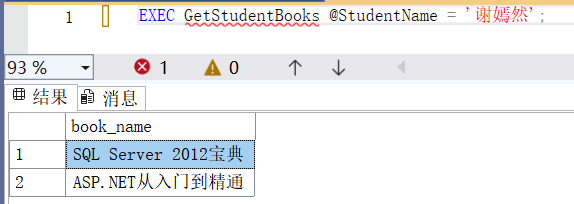
\includegraphics[width=0.8\textwidth]{img/result_2_2.png}
    \caption{查找学生所读图书结果}
\end{figure}

\subsubsection{图书价格调整}

\paragraph{实验目标}
定义一个存储过程，根据discount参数调整图书价格。

\paragraph{代码实现}
\begin{lstlisting}[language=SQL]
CREATE PROCEDURE AdjustBookPrice        -- 创建存储过程，调整图书价格
    @Discount DECIMAL(3,2)
AS
BEGIN
    CREATE TABLE #TempBookPrice (       -- 创建临时表存储原始价格，避免相互影响
        book_id CHAR(8),                -- 修改为CHAR(8)匹配实际表结构
        original_price MONEY             -- 修改为MONEY类型匹配实际表结构
    );
    
    INSERT INTO #TempBookPrice (book_id, original_price)        -- 插入原始价格
    SELECT book_id, book_price FROM book;
    
    UPDATE book         -- 更新价格小于等于35的图书
    SET book_price = t.original_price * (1 + @Discount)
    FROM book b
    INNER JOIN #TempBookPrice t ON b.book_id = t.book_id
    WHERE t.original_price <= 35;
    
    UPDATE book         -- 更新价格大于55的图书
    SET book_price = t.original_price * (1 - @Discount)
    FROM book b
    INNER JOIN #TempBookPrice t ON b.book_id = t.book_id
    WHERE t.original_price > 55;
    
    DROP TABLE #TempBookPrice;      -- 删除临时表
    END

EXEC AdjustBookPrice @Discount = 0.1;       -- 调用存储过程，discount = 0.1
\end{lstlisting}

\paragraph{结果展示}
\begin{figure}[H]
    \centering
    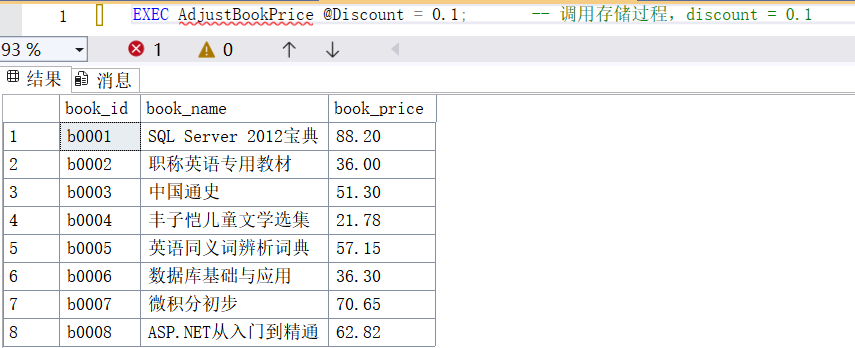
\includegraphics[width=0.8\textwidth]{img/result_2_3.png}
    \caption{图书价格调整结果}
\end{figure}

% 补充预期价格结果表格
\begin{center}
\begin{tabular}{ccc}
\toprule
book\_id & book\_name & 调整后预期价格 \\
\midrule
b0001 & SQL Server 2012宝典 & 98.00 $\times$ (1-0.1) = 88.20 \\
b0002 & 职称英语专用教材 & 36.00 \\
b0003 & 中国通史 & 57.00 $\times$ (1-0.1) = 51.30 \\
b0004 & 丰子恺儿童文学选集 & 19.80 $\times$ (1+0.1) = 21.78 \\
b0005 & 英语同义词辨析词典 & 63.50 $\times$ (1-0.1) = 57.15 \\
b0006 & 数据库基础与应用 & 33.00 $\times$ (1+0.1) = 36.30 \\
b0007 & 微积分初步 & 78.50 $\times$ (1-0.1) = 70.65 \\
b0008 & ASP.NET从入门到精通 & 69.80 $\times$ (1-0.1) = 62.82 \\
\bottomrule
\end{tabular}
\end{center}
和实际输出结果一致
\subsubsection{查找师承关系}

\paragraph{实验目标}
根据导师关系表，输入姓名，查找该学生的师承关系链。

\paragraph{代码实现}
\begin{lstlisting}[language=SQL]
CREATE TABLE advisor (                          -- 创建导师关系表
    MentorName VARCHAR(50) NOT NULL,            -- 导师姓名
    StudentName VARCHAR(50) NOT NULL            -- 学生姓名
);

INSERT INTO advisor (MentorName, StudentName) VALUES 
('Alice', 'Bob'),                           
('Alice', 'Carol'),                           
('David', 'Alice'),                            
('Mary', 'David'),                             
('Susan', 'Mary'),                            
('John', 'Susan');                             

CREATE FUNCTION GetAdvisorChain(@StudentName VARCHAR(50))       -- 创建递归查询函数，查找师承关系链
RETURNS VARCHAR(500)
AS
BEGIN
    DECLARE @Result VARCHAR(500) = '';
    
    WITH AdvisorChain AS (    -- 使用递归CTE查找师承关系链
        SELECT MentorName, 1 AS level
        FROM advisor
        WHERE StudentName = @StudentName
        
        UNION ALL
        
        SELECT a.MentorName, ac.level + 1
        FROM advisor a
        INNER JOIN AdvisorChain ac ON a.StudentName = ac.MentorName
    )
    SELECT @Result = COALESCE(    -- 将结果连接成字符串
        STUFF((
            SELECT ', ' + MentorName
            FROM AdvisorChain
            ORDER BY level
            FOR XML PATH(''), TYPE
        ).value('.', 'VARCHAR(MAX)'), 1, 2, ''),
        '无导师信息'
    );
    
    RETURN @Result;
END

-- 查询
SELECT dbo.GetAdvisorChain('Mary') AS AdvisorChain;      -- 结果应为Susan, John
\end{lstlisting}

\paragraph{运行结果}
\begin{figure}[H]
    \centering
    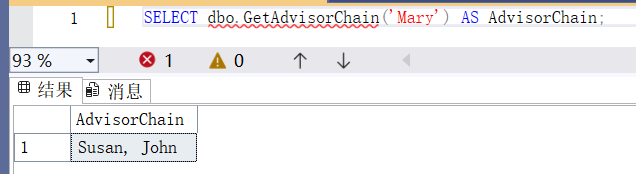
\includegraphics[width=0.8\textwidth]{img/result_2_4.png}
    \caption{师承关系查找结果}
\end{figure}

\subsection{游标实现图书总价计算}

\subsubsection{实验目标}
定义一个存储过程或函数，用游标的方式计算所有图书的总价。

\subsubsection{代码实现}
\begin{lstlisting}[language=SQL]
-- 创建存储过程，使用游标计算图书总价
CREATE PROCEDURE CalculateTotalPriceWithCursor
AS
BEGIN
    DECLARE @TotalPrice MONEY = 0;  -- 改为MONEY类型匹配表结构
    DECLARE @CurrentPrice MONEY;    -- 改为MONEY类型匹配表结构
    DECLARE @BookName VARCHAR(100);
    DECLARE @BookId CHAR(8);        -- 添加图书ID，匹配表结构
    
    -- 声明游标，包含图书ID和名称
    DECLARE book_cursor CURSOR FOR
    SELECT book_id, book_name, book_price FROM book;
    
    OPEN book_cursor;       -- 打开游标
    
    -- 获取第一条记录
    FETCH NEXT FROM book_cursor INTO @BookId, @BookName, @CurrentPrice;
    
    WHILE @@FETCH_STATUS = 0        -- 循环处理每条记录
    BEGIN
        SET @TotalPrice = @TotalPrice + @CurrentPrice;
        PRINT '图书ID: ' + @BookId + ', 名称: ' + @BookName + ', 价格: ' + CAST(@CurrentPrice AS VARCHAR(20));
        
        -- 获取下一条记录
        FETCH NEXT FROM book_cursor INTO @BookId, @BookName, @CurrentPrice;
    END
    
    CLOSE book_cursor;      -- 关闭游标
    DEALLOCATE book_cursor; -- 释放游标
    
    PRINT '所有图书总价: ' + CAST(@TotalPrice AS VARCHAR(20));
    SELECT @TotalPrice AS TotalPrice;
END

EXEC CalculateTotalPriceWithCursor;     -- 调用存储过程
\end{lstlisting}

\subsubsection{运行结果}
\begin{figure}[H]
    \centering
    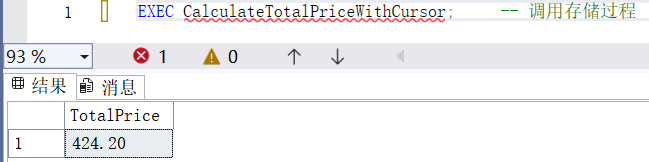
\includegraphics[width=0.8\textwidth]{img/result_3.png}
    \caption{使用游标计算图书总价结果}
\end{figure}

% 补充预期总价结果说明
\begin{center}
\textbf{预期总价：}
88.20 + 36.00 + 51.30 + 21.78 + 57.15 + 36.30 + 70.65 + 62.82 = 424.20
\end{center}
预期结果与输出一致
\subsection{实验总结}

\subsubsection{遇到的问题及解决方案}

在进行图书价格调整实验时，遇到了价格变化太大被阻止的问题。这是由于之前的实验中设置了触发器来限制价格的大幅变动。

\paragraph{问题描述}
执行价格调整存储过程时出现错误，系统阻止了价格的大幅变动。

\begin{figure}[H]
    \centering
    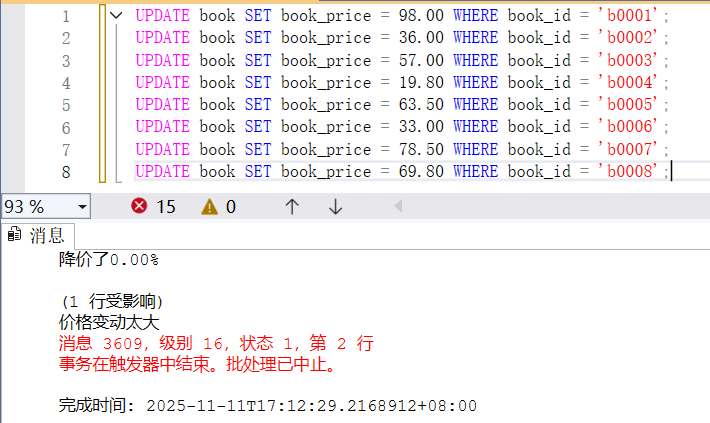
\includegraphics[width=0.8\textwidth]{img/problem1.png}
    \caption{触发器阻止价格变动错误截图}
\end{figure}

\paragraph{解决方案}
需要先查找并删除相关的触发器，然后重新执行价格调整操作。

\begin{lstlisting}[language=SQL]
-- 方案一：查找并删除触发器
-- 1. 先查找图书表上的触发器名称
SELECT 
    name AS TriggerName,                            -- 触发器名称
    OBJECT_NAME(parent_id) AS TableName,            -- 关联表名
    OBJECT_DEFINITION(object_id) AS TriggerDefinition   -- 触发器定义
FROM sys.triggers 
WHERE parent_id = OBJECT_ID('book');

-- 2. 找到触发器名称后，删除触发器
DROP TRIGGER tr_book_price_after;                  -- 删除价格变动限制触发器

-- 方案二：临时禁用触发器（如果需要保留触发器）
DISABLE TRIGGER tr_book_price_after ON book;    -- 禁用触发器

\end{lstlisting}

\paragraph{问题2：SQL Server函数创建与调用批处理分隔问题}

在SQL Server中，CREATE FUNCTION语句必须单独作为一个批处理，不能与其他语句（如SELECT）放在一起，否则会报语法错误。例如：

\begin{lstlisting}[language=SQL]
CREATE FUNCTION GetStudentInfo()
RETURNS VARCHAR(50)
AS
BEGIN
    RETURN '马福泉+23336179'
END
-- 调用函数
SELECT dbo.GetStudentInfo() AS StudentInfo;
\end{lstlisting}
上述写法会报错，因为CREATE FUNCTION和SELECT语句没有用GO分隔。
\paragraph{解决方案}
应将CREATE FUNCTION语句与调用语句分开，使用GO分隔批处理或者将调用语句放在另一个查询中：

\subsubsection{实验收获}

通过本次实验，我掌握了：
\begin{enumerate}
    \item 创建和调用无参数的存储过程和函数
    \item 创建带参数的存储过程和函数，实现复杂的业务逻辑
    \item 使用临时表避免数据更新时的相互影响
    \item 实现递归查询功能
    \item 使用游标遍历数据集进行计算
\end{enumerate}

存储过程和函数是数据库编程的重要工具，能够封装复杂的业务逻辑，提高代码的复用性和维护性。

\end{document}